\linespread{1.5}

O diagrama abaixo mostra a seção da parede de um forno. A face externa da parede está a temperatura ambiente de $20ºC$ e a face interna está a $600ºC$. Determine a função $u(x,t)$ que descreve a temperatura no interior da parede, sabendo-se que $u(x,t)$ é solução estacionário (invariante no tempo) da equação de difusão $u_t = a^2u_{xx}$, sendo $a^2$ a difusividade térmica da parede. 
\begin{figure}[H]
    \centering
    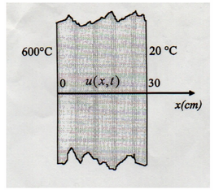
\includegraphics[width = 0.3\linewidth]{fig/edp17.png}
    \label{fig:edp17}
\end{figure}